\documentclass{acm_proc_article-sp}
%\usepackage{graphicx}
%\usepackage[pdftex]{graphicx}
\usepackage{subfig}
%\DeclareGraphicsExtensions{.pdf,.png,.jpg}
 \makeatletter
 \let\@copyrightspace\relax
 \makeatother

\begin{document}

\title{Mountain Skyline Recognition}



\numberofauthors{1} 
%
\author{
% 1st. author
\alignauthor
Matthew Beldyk\\
       \affaddr{University of Colorado}\\
       \affaddr{CSCI 5722}\\
       \affaddr{Boulder, Colorado}\\
       \email{beldyk@colorado.edu}
}

\maketitle
\begin{abstract}
Put abstract here
\end{abstract}

\section{Introduction}
A hiker often finds themselves looking at a mountain and wondering what that peak or other interesting geological feature is called.  The hiker is also often carrying a smart phone equipped with a GPS unit, Internet and a camera.  Using publicly available datasets and simple image processing techniques, I have attempted to create a system that answers that question within the constraints of the sensors a hiker would likely have in their cellular phone.  
\section{Body}
\subsection{The Current State of the Art}
There are a number of systems that currently do similar things to what my project attempts to achieve.  Marmota currently does everything my system attempts to do, but uses a much richer feature set than what I am attempting to utilize.\cite{chippendale2009environmental, chippendale2009spatial}  heywhatsthat.com is a website that creates the skyline render from DEMs and allows the user to manually identify the skyline they are wondering about \cite{wong2008we, heywhatsthat}.  This website only renders the skyline and annotates the model skyline, it does not annotate photographs.  The most relevant research that I’ve found is Behringer’s work \cite{behringer2002registration} where he uses the photograph and DEM skyline alignments as a way to augment other sensors in his system.  Behringer created a system quite similar to what I’ve attempted to create. I reused a significant amount of the math from Behringer’s paper in my research.

\subsection{Overview of the Algorithm}
	The basic flow of this algorithm is fairly simple, there are only a couple steps to calculate interesting results.  The first step is to calculate a number of parameters to set up the system.  First, latitude and longitude where the photograph is take must be calculated.  The next step is to load the DEM that corresponds to this location and calculate the elevation at this location.  Once the system has the coordinates for the location and the DEM is loaded into RAM, an optimal model 360 skyline must be rendered. 
	After this, the skyline in the photograph must be calculated.  The photograph is decimated and several filters are ran on the image to calculate the edge where the ground ends and the sky begins. Once both of these skylines are rendered, I treat them as waveforms \cite{Schafer:DSP} and try to find where the photograph's window best fits the model skyline. 
\subsection{Rendering from Model}
The first step in my algorithms is to create a model skyline from some geodetic dataset.  I decided to use the  SRTM 30M DEM dataset as the basis of my model of the skyline.  The SRTM dataset provides 1 lat by 1 lon square tiles that each contain a 3601x3601 matrix of elevations to meter resolution. \cite{farr2007shuttle} This is a simple format to read, but care must be taken to make sure that the corners of the tiles are aligned properly and that the tile is not being read backwards. If either of these cases happen the error is not immediately apparent, and can easily cascade later into the system.  
\begin{figure}
	\centering
	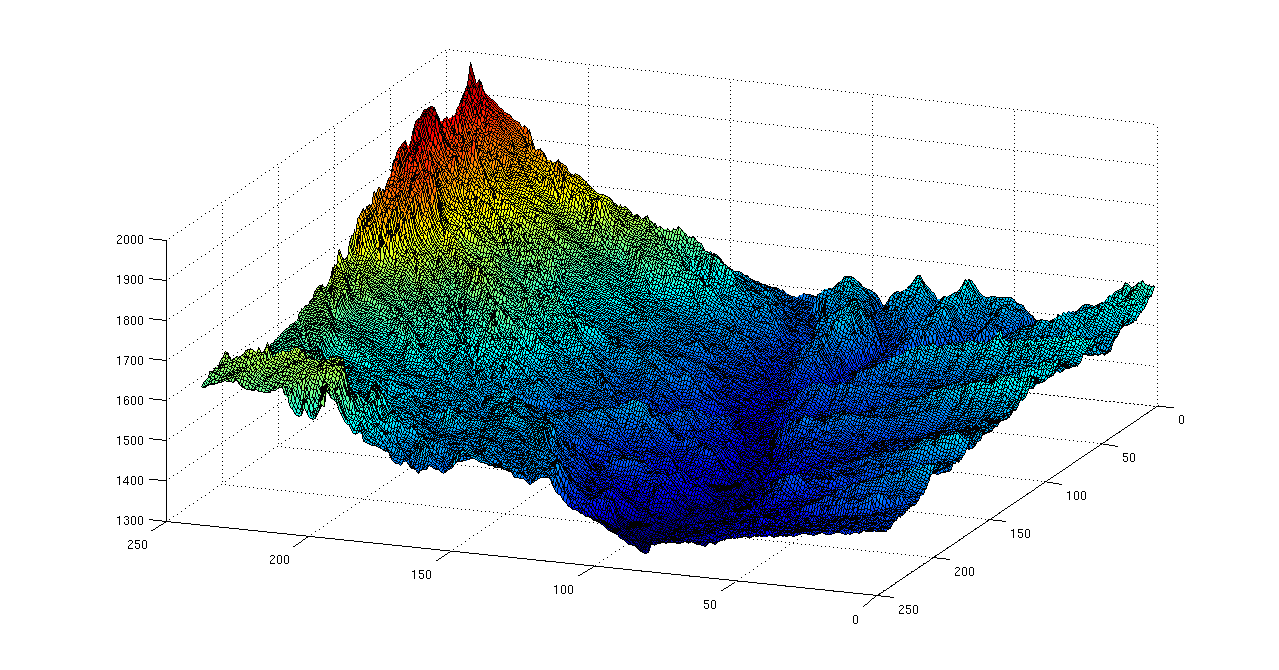
\includegraphics[width=0.5\textwidth]{boulderDem.png}
	\caption{An example of the decimated SRTM DEM for the area nearby Boulder, Colorado (the N40W105 tile.)}
	\label{fig:bldrDem}
\end{figure}

When I create my render, I load the DEM for the location where the photograph was taken.   If my location is too close to the edge of the DEM tile, I also need to render  neighbor tiles.  Once I have my DEM loaded, I need to render a full 360 view around where the photo was shot.  

To create this render, I use an algorithm similar to ray tracing.  I create a blank image that represents this view.  So that I can deal with less normalization issues later, I take the field of view of my photo (online one can look up the field of view parameters for a given camera for it’s various settings) and the number of pixels it is wide and tall to decide what size the 360 view model should be.  There are limitations to the amount of ram in the computer for this render, so this 360 view should not be too large, so the image must be decimated.

For every point in the DEM tile(s), I project this point into the image space.  I look at the point’s elevation and location to calculate the angle where it belongs in my render.  FIXME(equation here) I store the latitude, longitude and distance from the camera for each pixel (mostly for future extensions of this work.) During this projection, I felt it would be important to give precedence to closer items in each image pixel, so I do a check to see if the newest point is closer than the point currently projected into the same pixel.  In some future version of this algorithm, it might make sense to look at other features that appear from one mountain in front of another, instead of simply the ground/sky edge. For example, with this mode of rendering, I might be able to also annotate mountains in my foreground or use canyons and gullies as features in a future version of this system.

There are a number of issues that arise with this approach.  The first one noticed is that all of the points in the DEM are just that: points.  The skyline will result in a jagged edge that is not particularly useful for this system.  I solved this approach by asserting that each point would represent a window halfway to it’s neighbors.  The azimuth for each point becomes a window calculated by taking the maximum and minimum angles calculated by adding ½ the distance to the neighboring points to the point I am attempting to render.  This approach creates a more realistic render that looks as if I am rendering a series of square tiles instead of a cloud of points; it also has the advantage that it makes closer items look larger and farther items look smaller.  I then fill in the values for this specific point between the minimum and maximum azimuths found. FIXME(Equation here)
    Once I have rendered the entire skyline, I need to calculate the actual skyline waveform.  The algorithm to do this is much simpler than in the photo, I simply find the highest defined pixels in the image and store these values and their angle in the rendered image. These will be use at a later stage.

\subsection{Finding Skylines in Photos}
    There are numerous ways to find the edge where the ground meets the sky in a photograph.  I tried several convolution based methods, before I finally found one that suited my purposes:  a horizontal Sobel edge detector with some heuristic logic.  My initial testing involved using Matlab’s built in edge detectors \cite{mcandrew2004introduction} because it was trivial to try a large number of different filters quickly, but for my final version I wrote my own.  Initially, I tried a Canny edge detector, but it had too many false positives in the sky.  I next attempted to use several simple convolution \cite{Schafer:DSP} based filters of several different size, but most had too many false positives or simply did not find the skyline edge.  Finally, I settled on a 3x3 horizontal Sobel filter. \cite{behringer2002registration}  

As a preprocessing step, I decimate the image into one much smaller so that I have enough RAM in my machine to store the full 360 model render.  For my system, I decimate my photographs to 150 pixels wide; I found this to be a good compromise as large enough to still see features, but small enough that I wouldn’t use too much RAM for my model render. After I decimated, I would find the results of a convolution with a horizontal Sobel filter. Once I had the results from the convolution, I would apply a secondary filter to only keep filter responses above a certain threshold.\ref{fig:sobel}  After this filtration, I would search through each column of the image looking for the highest edge found; the relative elevation of these points in my image would be the skyline. \textbf{figs:annot} FIXME( put some images of annotated skylines and filter responses)
\begin{figure*}
	\centering
	  \subfloat[Original Image with Annotated Skyline]{
		\label{fig:org}
		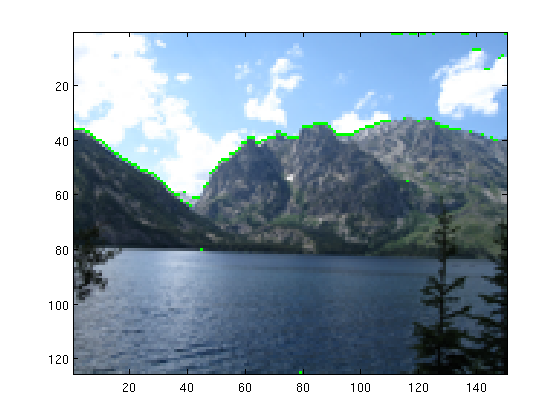
\includegraphics[width=0.5\textwidth]{picSkyline.png}}                	  
	\subfloat[Threasholded Sobel Responses]{
		\label{fig:sobel}
		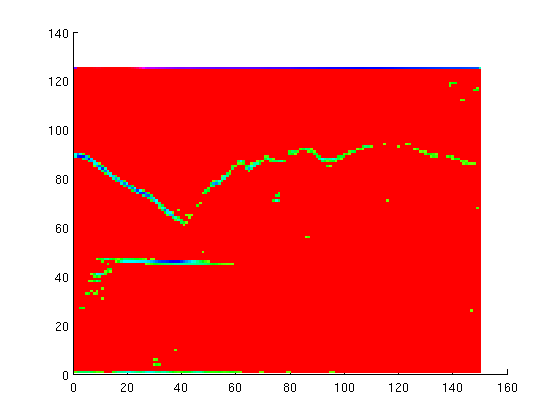
\includegraphics[width=0.5\textwidth]{picSobel.png}}                
	\caption{An example Sobel filter response}
\end{figure*}
\begin{figure*}
	\label{figs:annot}
	\centering
	\subfloat{\label{fig:night}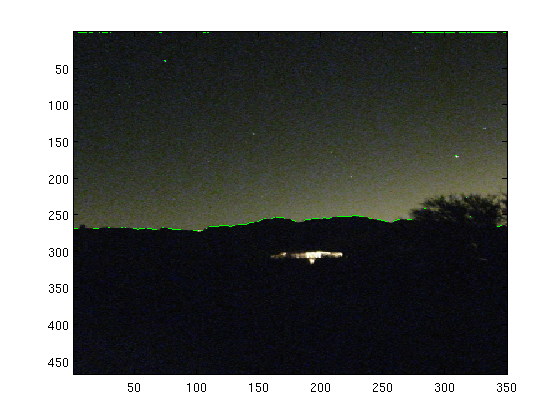
\includegraphics[width=0.3\textwidth]{nightAnnotated.png}}
	\subfloat{\label{fig:estes}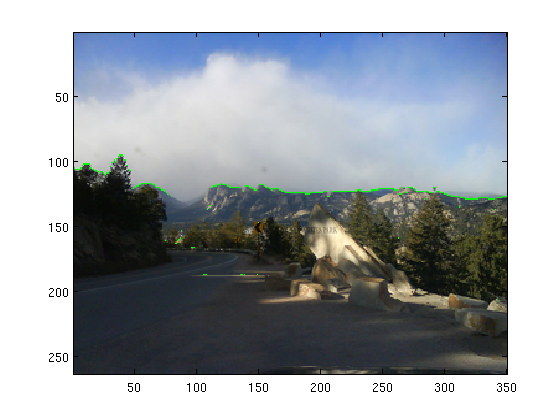
\includegraphics[width=0.3\textwidth]{estesParkAnnotated.png}}
	\subfloat{\label{fig:organPipes}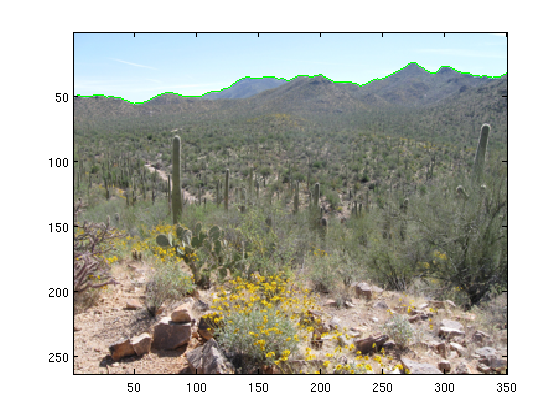
\includegraphics[width=0.3\textwidth]{organPipes2Annotated.png}}
	\caption{Several examples of good skyline edge finding}
\end{figure*}

    There are a number of assumptions in my code.  First, I make the assumption that the camera is upright, and the photograph was not taken at a strange angle.  I also make the assumption that there are no occlusions in the image, because they will appear as part of the skyline, and eventually throw off the entire eventual match.  This assumption is rather problematic, as it is rare to find a photograph with nothing nearby obscuring the full skyline, therefore cropping of images as a preprocessing step may be required. Figure \ref{fig:tetFail} shows an example of both occlusions and clouds. Another issue with my algorithm is that cumulonimbus and other fluffy white clouds create false positives for my algorithm.   Another problematic situation is a wide open plane with mountains in the far distance; my algorithm will miss the light blue mountains and find the edge between the plane and the mountains (see Figure \ref{fig:whiteSandsFail}.)  
\begin{figure}
	\centering
	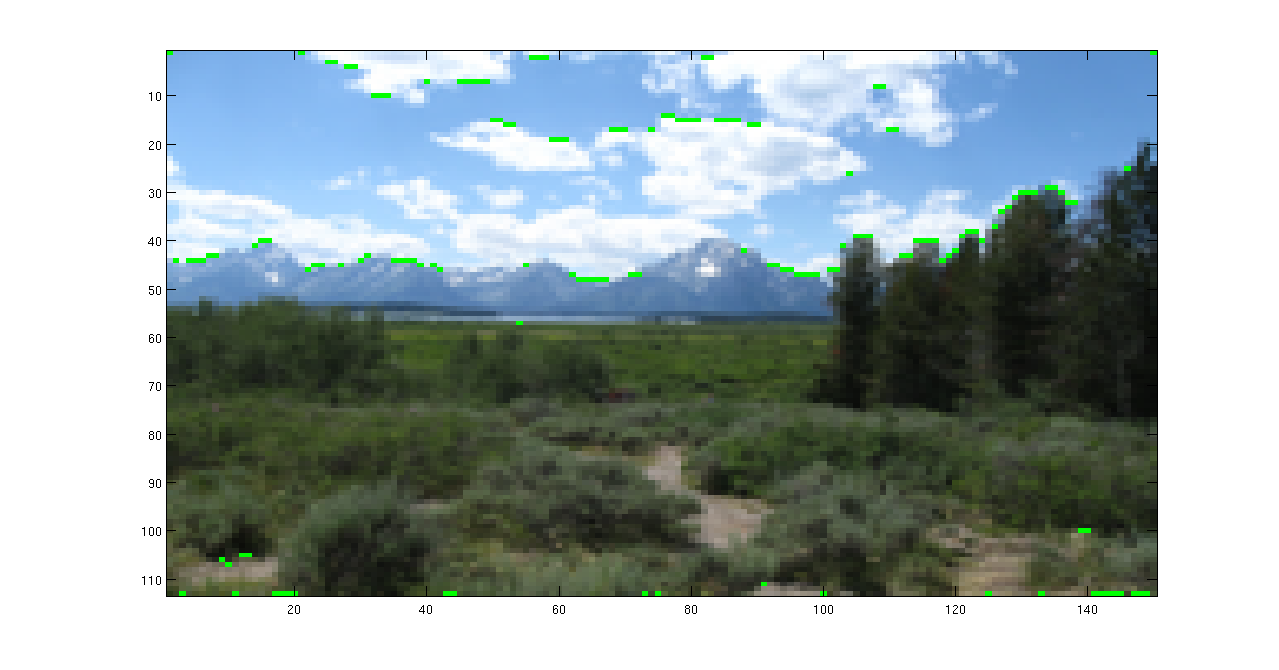
\includegraphics[width=0.5\textwidth]{tetonsCloudErrorSmallSkyline.png}
	\caption{An example of when my algorithm fails due to both clouds and occlusions.}
	\label{fig:tetFail}
\end{figure}
\begin{figure}
\centering
	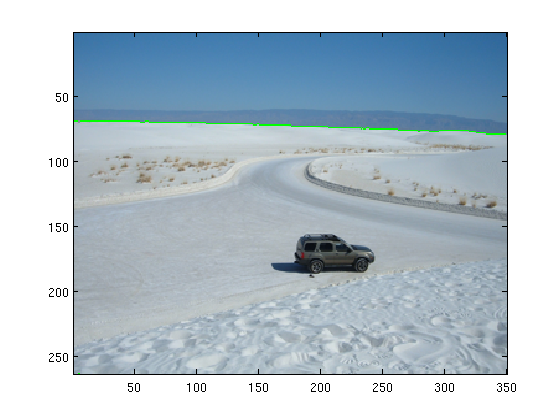
\includegraphics[width=0.5\textwidth]{whiteSandsAnnotated.png}
	\caption{An example of when my algorithm fails due a weak response of the actual skyline.}
	\label{fig:whiteSandsFail}
\end{figure}

\subsection{Matching the Photograph Skyline with the Model Skyline}
    Once the two skylines have been calculated, the subwindow that the photograph viewport represents must be matched with the corresponding view in the model skyline.  The literature suggests using local maximums and minimums (small peaks and valleys in the skyline) as features to match. My approach was to treat the entire skyline  waveform from the photo as a feature vector with a number of missing data points. At this point I have some waveform that goes through the photograph at some elevation in the field of view.  I need to normalized this waveform’s absolute angles to some relative angle.  I choose the median angle of all the skyline points that are actually defined, and then I subtract this median angle from the absolute angle in the skyline to create a new skyline with a median of zero.  I would then iterate over the entire model skyline looking at every possible window in a 360 view around the model skyline.  Each hypothesis window is normalized in the same way that I normalized the photo skyline, thus I am comparing two similar feature vectors.  My algorithm then looks for the closest match using a modified Euclidean distance, but ignoring the pixels in the feature vectors where they are undefined in the photograph skyline.  Once I’ve found the best match in the model skyline, I then need map the pixel coordinates back to the actual angles of the field of view.
\section{Results}
    In the end, I did not have enough time to create a completely working system.  The final code for matching the two skylines that I created has a bug in it that is returning wrong results.  I believe it to be something trivial, but there is no longer any time in the semester to complete debugging the codebase.  Once that bug is fixed, the next step is to project interesting visible geological features into the photograph and annotating the image.
    This said, I was successful in creating a system that was able to find the shape skyline edge in all but two of the 30 images in my test set.  I also created a system that can create a skyline from a model in a fairly quick amount of time (a full undecimated run of the entire system takes under 20 minutes on a 2.2GHz AMD Turion.)  Slightly decimated versions of the dataset run significantly faster; with a minimal amount of decimation, the loading of the 25MB SRTM datafile from the filesystem becomes the largest bottleneck.  
future work
\subsection{Future Work}
    The code created in the project is a great start for an augmented reality mobile application that solves the problem I initially intended to solve.  In a real version of the system, other ancillary sensors would be utilized to improve the accuracy of the identification.  For example, many cellphones that contain GPS units also contain a digital compasses, tilt meters, and accelerometers which may be accurate enough to no longer need to do computer vision identification of the skyline.  In fact, I intent to take much of what I’ve learned with this project to create an augmented reality cellphone application that identifies mountains this winter break, but I do plan to utilize these other external sensors to cut down on processor time.





%\begin{figure}
%\centering
%\epsfig{file=fly.eps}
%\caption{A sample black and white graphic (.eps format).}
%\end{figure}

\section{Conclusions}
This paragraph will end the body of this sample document.

\bibliographystyle{abbrv}
\bibliography{computer_vision_paper}


\end{document}